\documentclass[legalpaper,11pt,extrafontsizes,oneside,openany,x11names]{memoir}

\usepackage{geometry}
\geometry{portrait,left=1in,right=1in,top=1in,bottom=1in}
\setlength{\columnsep}{20pt}

\usepackage{amsmath}
\usepackage{booktabs}

\usepackage{graphicx}
\usepackage{caption}

\usepackage{multicol}
\usepackage{enumitem}
\usepackage{titlesec}

\usepackage{fancyhdr}
\fancypagestyle{plain}{
    \fancyhead[L]{\sffamily \textbf{LAKI, Tamira Marie A.}} 
    \fancyhead[C]{\sffamily \textbf{Math Modeling (MAT305)}}
    \fancyhead[R]{\sffamily \textbf{BSM CS 3A-G2}}
    \fancyfoot[C]{\thepage}
}

\usepackage{xcolor}
\usepackage{listings}
\definecolor{codegray}{rgb}{0.9,0.9,0.9}

\lstset{
    backgroundcolor=\color{codegray},
    basicstyle=\ttfamily\small,
    breaklines=true,
    frame=single,
    captionpos=b,
    language=Matlab
}

\setlength{\itemsep}{0pt}
\setlength{\topsep}{0pt}
\setlength{\parsep}{0pt}
\setlength{\parskip}{0pt}

\titlespacing*{\section}{0pt}{1.5ex plus .2ex minus .2ex}{1ex plus .2ex}
\titlespacing*{\subsection}{0pt}{1.5ex plus .2ex minus .2ex}{0.5ex plus .2ex}
\titlespacing*{\subsubsection}{0pt}{1.5ex plus .2ex minus .2ex}{0.5ex plus .2ex}

\parindent0in
\pagestyle{plain}
\thispagestyle{plain}

\makeatletter
\def\maketitle{
    \begin{center}
        \LARGE \textbf{\@title} \\[0.5ex]
        \large \@date
    \end{center}
}
\makeatother

\title{Activity - Cubic Splines}
\date{May 3, 2025}

\setcounter{section}{0}
\renewcommand{\thesection}{\arabic{section}}

\begin{document}
\maketitle

\section*{Problem}

Given the data set below, write a system of equations to determine the coefficients of the natural cubic splines passing through the data points. Construct the natural spline model and graph the splines together with the data points.

\[
\begin{array}{|c|c|c|c|}
\hline
x_i & 2 & 4 & 7 \\
\hline
y_i & 2 & 8 & 12 \\
\hline
\end{array}
\]

\section*{Solution}

\[
\begin{aligned}
S_i(x) &= y_i : \\
S_1(x) &= a_1 + b_1x + c_1x^2 + d_1x^3, \quad x \in [2,4] \\
a_1 + 2b_1 + 4c_1 + 8d_1 &= 2 \\
S_2(x) &= a_2 + b_2x + c_2x^2 + d_2x^3 \\
S_3(x) &= a_3 + b_3x + c_3x^2 + d_3x^3 \\
S_4(x) &= a_4 + 7b_4 + 49c_4 + 343d_4 = 12 \\
S_1'(x) &= b_1 + 2c_1x + 3d_1x^2, \quad x \in [2,4] \\
2c_1 + 6d_1(4) &= 2c_2 + 6d_2(4) \\
b_2 - b_1 &= 8c_1 + 48d_1 - 8c_2 - 48d_2 = 0 \\
2c_1 + 24d_1 - 2c_2 - 24d_2 &= 0 \\
2c_1 + 12d_1 &= 0 \\
2c_4 + 12d_4 &= 0
\end{aligned}
\]

\section*{Linear Algebraic System of Equations}

\[
\begin{aligned}
a_1 + 2b_1 + 4c_1 + 8d_1 &= 2 \\
a_1 + b_1 + c_1 + d_1 &= 2 \\
a_1 + 6b_1 + 36c_1 + 216d_1 &= 0 \\
a_1 + 7b_1 + 49c_1 + 343d_1 &= 2 \\
a_2 + 8b_2 + 64c_2 + 512d_2 &= 2 \\
b_2 + 8c_2 + 96d_2 - 8c_2 - 96d_2 &= 0 \\
2c_1 + 12d_1 - 2c_2 - 12d_2 &= 0 \\
2c_1 + 12d_1 &= 0 \\
2c_2 + 42d_2 &= 0
\end{aligned}
\]

\section*{Matrix}

\[
\begin{array}{cccccccc|c}
a_1 & b_1 & c_1 & d_1 & a_2 & b_2 & c_2 & d_2 & \\
\hline
1 & 2 & 4 & 8 & 0 & 0 & 0 & 0 & 2 \\
1 & 1 & 1 & 1 & 0 & 0 & 0 & 0 & 2 \\
1 & 6 & 36 & 216 & 0 & 0 & 0 & 0 & 0 \\
1 & 7 & 49 & 343 & 0 & 0 & 0 & 0 & 2 \\
0 & 0 & 0 & 0 & 1 & 8 & 64 & 512 & 2 \\
0 & 0 & 0 & 0 & 0 & 1 & 0 & 0 & 0 \\
0 & 0 & 2 & 12 & 0 & 0 & -2 & -12 & 0 \\
0 & 0 & 2 & 12 & 0 & 0 & 0 & 0 & 0 \\
0 & 0 & 0 & 0 & 0 & 0 & 2 & 42 & 0 \\
\end{array}
\]

\[
\begin{aligned}
a_1 &= -4 \\
b_1 &= 2.3333 \\
c_1 &= 0.5 \\
d_1 &= -0.0833 \\
a_2 &= -12.8888 \\
b_2 &= 0 \\
c_2 &= 1.6666 \\
d_2 &= -0.0555 \\
\end{aligned}
\]

\section*{Interval Model}

\[
\begin{array}{ll}
2 \leq x < 4 & S_1(x) = -4 + 2.333x + 0.5x^2 - 0.0833x^3 \\
4 \leq x \leq 7 & S_2(x) = -12.8888 + 9x - 1.6666x^2 + 0.0555x^3 \\
\end{array}
\]

\section*{MATLAB Code}
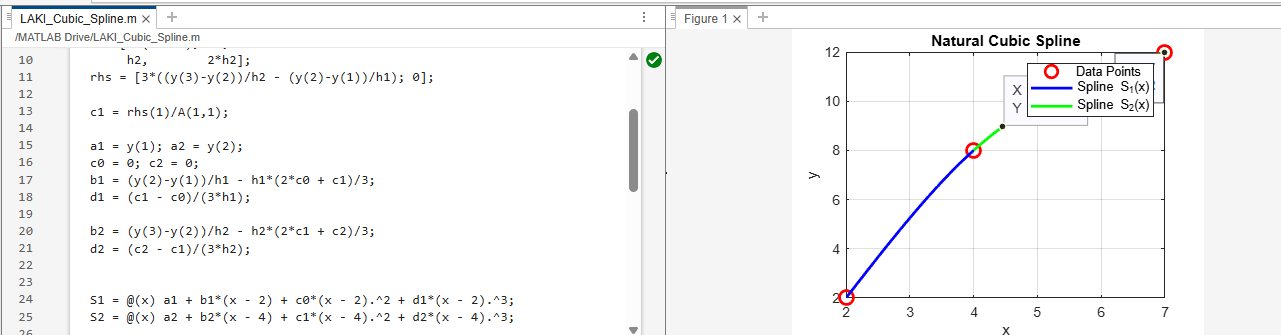
\includegraphics[width=\textwidth]{assets/cspline.png}

\end{document}
